\documentclass[a4paper,12pt]{article}
\usepackage{graphicx}
\usepackage[left=30mm, right=30mm, top=30mm, bottom=30mm]{geometry}
\usepackage{amsmath}
\usepackage{siunitx}
\usepackage{fancyhdr}
\usepackage{url}
\pagestyle{fancy}
%-------------------------------------------------------------------------------
\lhead{\textbf{Spring 2019}}
\rhead{\textbf{CE394M Advanced Analysis in Geotechnical Engineering}}
\cfoot{\thepage}
%-------------------------------------------------------------------------------

\begin{document}
\begin{centering}
	\textbf{
		Assignment 7: Linear Elastic Finite Element Analysis\\
		Assigned: 17th April 2019\\
		Due: 26th April 2019\\
	}
\end{centering}

\vspace{1em}
 
\begin{enumerate}

	\item     1. Using the finite element program PLAXIS 2D, analyze the response of an isotropically consolidated triaxial specimen under drained loading in triaxial compression.  PLAXIS 2D includes a module that uses the specified constitutive model parameters to predict the results from common laboratory tests.  This Soil Test option is found under the Material Sets window and is further explained in Section 6.3 of the Reference Manual.  
	
	For this assignment, use the consolidated-drained triaxial test data for a sand found in hw3-tx-data.xlsx posted on Canvas.  Assume that the soil can be modeled as a linear elastic material.  Select a linear elastic material using PLAXIS and assign its properties by the elastic parameters $E$ and $\nu$.  For the baseline case, use the TX test data to define a secant Young's modulus over an axial strain range of about 0 to 0.5\%.  Use this value of $E (E_{0.5\%})$ along with $\nu = 0.2$.  The soil's unit weight should be set to 18 kN/m3, although this value will not be used in the triaxial test simulation.  Isotropically load the triaxial specimen to a confining stress of 100 kPa, and compute the response up to an axial strain of 5\%.  
	
	\begin{enumerate}
		\item For this baseline case ($E_{0.5\%}$ and $\nu = 0.2$), plot the results in the familiar deviator stress ($q = \sigma_1 - \sigma_3$) vs. axial strain and volumetric strain vs. axial strain format.  Check the strain results from PLAXIS with a hand calculation using the equations of isotropic, linear elasticity.  Compare the predicted curves with those from the triaxial test.  Comment on the applicability of the model to the triaxial test data.
		\item Run three additional analyses with the following properties: (1) Define a secant $E$ over the strain range from 0 to 2.0\% (E2.0\%) and $\nu = 0.2$, (2) $E = E_{0.5\%}$ (baseline value) and $\nu = 0.4$, and (3) determine $E_{50}$ and $\nu = 0.2$  Discuss how changing $E$ and $\nu$ affects the results.
		\item Using the baseline properties, run an undrained triaxial test by selecting Undrained as the type of test.  Plot deviator stress vs. axial strain and volumetric strain vs. axial strain, and compare these results with those obtained for drained conditions in (a).  Explain any differences.
	\end{enumerate}
	
	\item Using the finite element program PLAXIS 2D, analyze the plane strain problem of a long strip surface loading of a linear elastic finite layer underlain by a rigid base (see figure below).  There is no water; hence, effective stresses equal total stresses.  Note that for this problem: $E = 20,000 kPa, \nu = 0.2, H = 10 m, q = 250 kPa$, and $B = 3 m$.  You can select a linear elastic material using PLAXIS and assign its properties by the elastic parameters E and $\nu$.  The soil's unit weight should be set to zero, so that the results can be compared to elastic solutions for the effect of the addition of the surface load only.  You will still need to calculate initial stresses with PLAXIS, but they will be zero.  The soil is treated as an existing foundation and the surface load as an applied distributed load.  Start by using a ``coarse'' mesh of 15-node triangles as the finite element model in this analysis.  Show a plot of the finite element mesh used in your baseline analysis with the boundary conditions and the deformed mesh for the baseline case.  Examine the results from the FE analysis to observe the distribution of displacements and stresses across the region. Specifically:
	
	\begin{enumerate}
		\item Compare the vertical and horizontal displacements at the edge of the strip loading predicted by PLAXIS and the elastic solutions of Poulos and Davis (1974), which are attached.  
		
		\item Compare the vertical stress versus depth beneath the edge of the strip loading predicted by PLAXIS and Poulos and Davis (1974).
		
		\item Evaluate the sensitivity of the results (i.e., vertical and horizontal displacements at the edge of the loading and the vertical stress distribution beneath the edge) to the finite element model employed in the analysis by re-analyzing the baseline case using a ``very coarse'' mesh of 6-node triangles and a ``very fine'' mesh of 15-node triangles.
		
		\item Evaluate the sensitivity of the results to variations in the two elastic parameters E and $\nu$. Specifically, perform analyses with (1) $E = 40,000 kPa$ and $\nu= 0.2$, and (2) $E = 20,000 kPa$ and $\nu = 0.4$.
		
		\item Evaluate the sensitivity of the results to variations in the thickness of the soil layer (H) by performing analyses with $H = 5 m$ and $20 m$.
	\end{enumerate}

	\begin{figure}[!h]
		\centering
		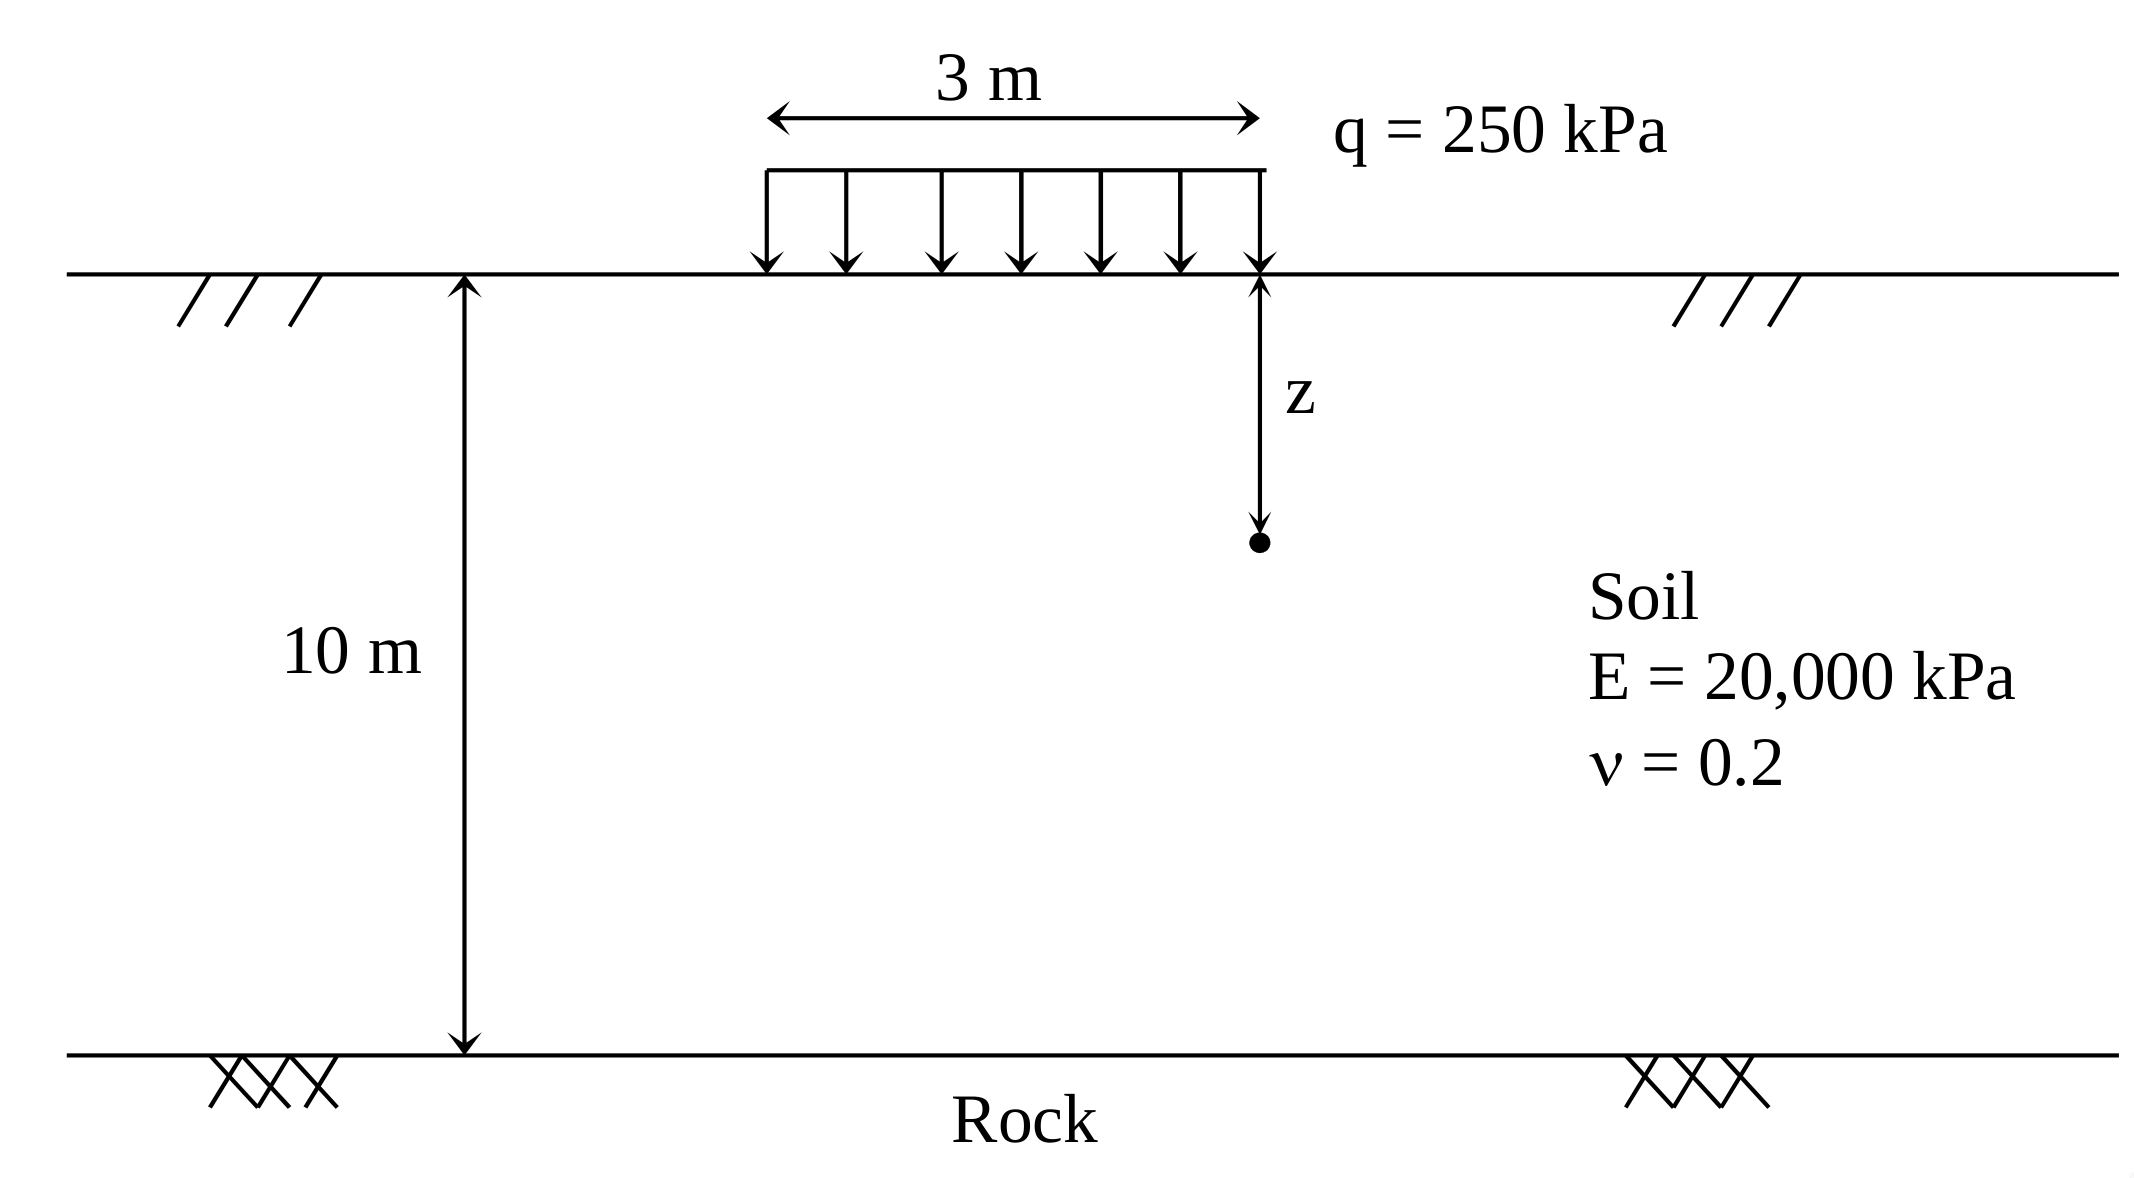
\includegraphics[width=0.85\textwidth]{figs/footing.png}
	\end{figure}
\end{enumerate}

\end{document}

